\documentclass[11pt]{article}
\usepackage{certmachine}
\usepackage{graphicx}
%% generated by tools/paper-numbers/ramsey-chain.js from certs/gnnw-certificate.json, certs/gnnw-chain-certificate.json, corpus/gnnw, instruments/gnnw/propose, certs/horizonmath-ledger.json, corpus/horizonmath — do not edit (git eece01c1497a)
\newcommand{\RepoCommit}{eece01c1497a}
\newcommand{\GnnwArxiv}{2407.19026v2}
\newcommand{\GnnwSha}{2d5be61d0442}
\newcommand{\GnnwVoneSha}{148e722db641}
\newcommand{\VerifierSha}{996c82c5500c}
\newcommand{\SecondSha}{9012c15a194f}
\newcommand{\ChainSha}{4912112b1b17}
\newcommand{\ZGenerated}{2026-09-29}
\newcommand{\KGenerated}{2026-09-29}
\newcommand{\SecondRan}{2026-09-29}
\newcommand{\PrecisionPy}{40}
\newcommand{\PrecisionJs}{120}
\newcommand{\QaiPoly}{-0.3864\lambda + 0.8347\lambda^{2} - 2.0156\lambda^{3} + 2.7171\lambda^{4} - 1.7541\lambda^{5} + 0.4522\lambda^{6}}
\newcommand{\QaiSum}{-0.1521}
\newcommand{\PrintedBase}{3.78233}
\newcommand{\PrintedIs}{its rounding}
\newcommand{\CroundOne}{3.7823287755373116}
\newcommand{\CroundOneFull}{3.7823287755373116217428004578}
\newcommand{\CroundOneSix}{3.782328}
\newcommand{\MzeroOne}{1.505717}
\newcommand{\MN}{100}
\newcommand{\MNodes}{101}
\newcommand{\MLast}{0.392143}
\newcommand{\MaxM}{0.3928}
\newcommand{\MinFp}{0.756}
\newcommand{\TailOne}{79}
\newcommand{\MainOne}{336}
\newcommand{\IntervalsOne}{415}
\newcommand{\MinTailSOne}{$4.72\times10^{-6}$}
\newcommand{\MinMainLowerOne}{$9.55\times10^{-7}$}
\newcommand{\WorstLo}{0.6875}
\newcommand{\WorstHi}{0.69}
\newcommand{\SecondsOne}{7.6}
\newcommand{\RemarkPre}{We asked ChatGPT 5.6 Sol to perform an additional iteration of optimization in Theorem 14. A preliminary, unverified iteration suggests that Theorem 1 holds with}
\newcommand{\RemarkPost}{If verified it would improve the upper bound on the diagonal Ramsey numbers to $R(k,k)\le(3.78233\ldots)^{k+o(k)}$. Further improvements by performing additional iterations are possible, but we expect that lowering the base of the exponent below 3.7 and, likely, even below 3.75 would require new ideas.}
\newcommand{\RemarkPage}{20}
\newcommand{\CurveN}{160}
\newcommand{\SlackLim}{$6.31\times10^{-5}$}
\newcommand{\SlackMin}{$6.20\times10^{-5}$}
\newcommand{\SlackMinAt}{0.93}
\newcommand{\SlackLimM}{6.31\times10^{-5}}
\newcommand{\SlackMinM}{6.20\times10^{-5}}
\newcommand{\SlackMax}{0.0373}
\newcommand{\SlackMaxAt}{0.11}
\newcommand{\SlackAtOne}{$3.56\times10^{-4}$}
\newcommand{\NRounds}{6}
\newcommand{\NNew}{5}
\newcommand{\DegNew}{9}
\newcommand{\DegOne}{6}
\newcommand{\RegionVerdict}{strictly concave and increasing on (0, 1]; A < B}
\newcommand{\AgreeDigits}{25}
\newcommand{\CFinalPy}{3.7721307629003663892468671139}
\newcommand{\CFinalJsLo}{3.7721307629003663892468671}
\newcommand{\CFinalJsHi}{3.7721307629003663892468672}
\newcommand{\BaseFinalTen}{3.7721307629}
\newcommand{\BaseFinalFour}{3.7721}
\newcommand{\BaseFinalSix}{3.772130}
\newcommand{\BaseFinalFive}{3.77213}
\newcommand{\BaseFinalUp}{3.7722}
\newcommand{\BaseTwoSix}{3.775471}
\newcommand{\BaseThreeSix}{3.772573}
\newcommand{\BaseFourSix}{3.772275}
\newcommand{\BaseFiveSix}{3.772151}
\newcommand{\BasesArrow}{3.782328 $\to$ 3.775471 $\to$ 3.772573 $\to$ 3.772275 $\to$ 3.772151 $\to$ 3.772130}
\newcommand{\IntervalsPyTotal}{4{,}059}
\newcommand{\IntervalsJsTotal}{181{,}977}
\newcommand{\SecondsChainPy}{176}
\newcommand{\MinutesChainJs}{35}
\newcommand{\SecondsChainJs}{2{,}099}
\newcommand{\DeltaMargin}{$5\times10^{-5}$}
\newcommand{\DeltaMarginM}{5\times10^{-5}}
\newcommand{\GridPoints}{215}
\newcommand{\ChainRows}{1 & 6 & 1.505717 & 3.78232877553731 & 3.7823287755373116217428004 \\
2 & 9 & 1.496675 & 3.77547102153684 & 3.7754710215368457179220446 \\
3 & 9 & 1.491435 & 3.77257346178090 & 3.7725734617809080648710855 \\
4 & 9 & 1.491432 & 3.77227508535433 & 3.7722750853543349625183954 \\
5 & 9 & 1.491370 & 3.77215157829815 & 3.7721515782981542341194064 \\
6 & 9 & 1.491363 & 3.77213076290036 & 3.7721307629003663892468671 \\}
\newcommand{\IntervalRows}{1 & 79 & 336 & $4.7\times10^{-6}$ & $9.6\times10^{-7}$ & 79 & 11{,}322 & $4.7\times10^{-6}$ & $3.7\times10^{-8}$ \\
2 & 10 & 693 & $3.6\times10^{-4}$ & $1.4\times10^{-7}$ & 10 & 39{,}820 & $3.0\times10^{-4}$ & $2.3\times10^{-10}$ \\
3 & 16 & 736 & $4.9\times10^{-4}$ & $6.6\times10^{-8}$ & 16 & 34{,}758 & $4.6\times10^{-4}$ & $1.3\times10^{-11}$ \\
4 & 12 & 718 & $7.1\times10^{-4}$ & $1.0\times10^{-7}$ & 12 & 31{,}982 & $6.7\times10^{-4}$ & $5.4\times10^{-10}$ \\
5 & 12 & 717 & $4.7\times10^{-4}$ & $1.7\times10^{-7}$ & 12 & 31{,}713 & $4.3\times10^{-4}$ & $2.2\times10^{-10}$ \\
6 & 12 & 718 & $5.3\times10^{-4}$ & $1.0\times10^{-8}$ & 12 & 32{,}241 & $4.9\times10^{-4}$ & $3.8\times10^{-11}$ \\}
\newcommand{\CoeffRows}{1 & $-0.3864$ & $0.8347$ & $-2.0156$ & $2.7171$ & $-1.7541$ & $0.4522$ & --- & --- & --- \\
2 & $-0.416545$ & $0.646462$ & $0.255568$ & $-4.938579$ & $10.000000$ & $-7.007958$ & $-1.007665$ & $3.557723$ & $-1.246039$ \\
3 & $-0.434002$ & $0.835266$ & $-0.514657$ & $-3.672465$ & $10.000000$ & $-10.000000$ & $3.360082$ & $0.894786$ & $-0.628130$ \\
4 & $-0.434013$ & $0.830597$ & $-0.499373$ & $-3.688645$ & $10.000000$ & $-10.000000$ & $3.384087$ & $0.866940$ & $-0.618928$ \\
5 & $-0.434220$ & $0.831682$ & $-0.501864$ & $-3.686634$ & $10.000000$ & $-10.000000$ & $3.382308$ & $0.868797$ & $-0.619493$ \\
6 & $-0.434241$ & $0.831665$ & $-0.501774$ & $-3.686715$ & $10.000000$ & $-10.000000$ & $3.382333$ & $0.868789$ & $-0.619496$ \\}
\newcommand{\FloatBox}{10}
\newcommand{\BoxActiveLast}{2}
\newcommand{\FloatSixIters}{5}
\newcommand{\FloatNineIters}{8}
\newcommand{\FloatSixLast}{3.773180}
\newcommand{\FloatNineLast}{3.7721261}
\newcommand{\FloatSixSettle}{3.7732}
\newcommand{\FloatNineSettle}{3.77213}
\newcommand{\FloatSixDrop}{$4.3\times10^{-5}$}
\newcommand{\FloatNineDrop}{$2.6\times10^{-7}$}
\newcommand{\FloatNineBeyond}{$4.6\times10^{-6}$}
\newcommand{\FloatRows}{0 & 3.782329 & 3.7823288 \\
1 & 3.775910 & 3.7754705 \\
2 & 3.773963 & 3.7725741 \\
3 & 3.773382 & 3.7722750 \\
4 & 3.773223 & 3.7721512 \\
5 & 3.773180 & 3.7721329 \\
6 & --- & 3.7721274 \\
7 & --- & 3.7721264 \\
8 & --- & 3.7721261 \\}
\newcommand{\HmArxiv}{2603.15617v2}
\newcommand{\HmSha}{9616325eadb6}
\newcommand{\HmCommit}{4ef0b61a}
\newcommand{\HmCommitFull}{4ef0b61a8a6d4c5ded661fab7c2e896af84abe6e}
\newcommand{\LGenerated}{2026-09-29}
\newcommand{\HmObservedOn}{2026-09-29}
\newcommand{\HmClaimant}{GPT-5.4 Pro, reproduced by GPT-5.6 Sol Max}
\newcommand{\HmCEncLo}{3.6960839126}
\newcommand{\HmC}{3.6960839126}
\newcommand{\HmCFour}{3.6960}
\newcommand{\HmCPrinted}{3.69608391263}
\newcommand{\HmUcubic}{-0.25\mu + 0.033\mu^{2} + 0.08\mu^{3}}
\newcommand{\HmQuintic}{-0.0778}
\newcommand{\HmCoeffs}{(-0.25,\,0.033,\,0.08,\,0,\,-0.0778)}
\newcommand{\HmShrinkPct}{0.12\%}
\newcommand{\HmShrink}{0.0012}
\newcommand{\HmLambdaZero}{10^{-3}}
\newcommand{\HmIntervals}{200}
\newcommand{\HmPoints}{201}
\newcommand{\HmOutside}{56}
\newcommand{\HmNotPlaced}{128}
\newcommand{\HmNotRefuted}{17}
\newcommand{\HmEU}{0.26292}
\newcommand{\HmEUlong}{0.26292279}
\newcommand{\HmChyp}{0.26292278641656774}
\newcommand{\HmLastX}{0.22745}
\newcommand{\HmLastXlong}{0.22745427}
\newcommand{\HmLastY}{0.9988}
\newcommand{\HmLastM}{0.3229}
\newcommand{\HmE}{13/2000}
\newcommand{\HmEdec}{0.0065}
\newcommand{\HmP}{11981/500000}
\newcommand{\HmPdec}{0.023962}
\newcommand{\HmErdosLo}{0.012127}
\newcommand{\HmPairHi}{0.010826}
\newcommand{\HmGap}{0.00130}
\newcommand{\HmFirstLambda}{0.00102}
\newcommand{\HmFirstX}{0.99769}
\newcommand{\HmFirstY}{0.26321}
\newcommand{\HmFirstE}{19/2000}
\newcommand{\HmFirstP}{8033/250000}
\newcommand{\HmNrLamLo}{0.236}
\newcommand{\HmNrLamHi}{0.374}
\newcommand{\HmNrXLo}{0.4365}
\newcommand{\HmNrXHi}{0.5988}
\newcommand{\HmCheckerSeconds}{107}
\newcommand{\HmCheckerLine}{299}
\newcommand{\HmWithAndSeconds}{0.2}
\newcommand{\HmFirstIntervalLo}{0.001}
\newcommand{\HmFirstIntervalHi}{0.0010014}
\newcommand{\HmCheckerOutput}{Valid split certificate; c = e\textasciicircum{}\{F(1)\} = 3.69608391263; polynomial\_coeffs degree = 5; analytic tail endpoint = 0.00010846; worst small-lambda slack = 0.000272305; worst large R\_0 slack = 0.000951234; worst large main slack = 0.000318787}
\newcommand{\HmCheckerMin}{return max(mp.mpf(0), min(bu, bs))}
\newcommand{\HmCheckerMax}{max(bu, bs)}
\newcommand{\HmAone}{0.4657}
\newcommand{\HmBone}{0.5645}
\newcommand{\HmSampleRows}{0.0010 & 0.99769 & 0.26321 & outside $R$ & $e = 19/2000$, $p = 8033/250000$: gap 0.00134 \\
0.0058 & 0.98706 & 0.26601 & not placed by $U$ & $s = 319/1000$: $U(s)$ exceeds the line by 0.2406 \\
0.0331 & 0.92892 & 0.28245 & not placed by $U$ & $s = 703/2000$: $U(s)$ exceeds the line by 0.2000 \\
0.1407 & 0.73107 & 0.35746 & not placed by $U$ & $s = 541/1000$: $U(s)$ exceeds the line by 0.0632 \\
0.3134 & 0.50087 & 0.52209 & not refuted here & --- \\
0.5725 & 0.26328 & 0.99325 & not placed by $U$ & $s = 157/500$: $U(s)$ exceeds the line by 0.2436 \\
0.8316 & 0.26070 & 0.99880 & outside $R$ & $e = 23/2500$, $p = 31483/1000000$: gap 0.00234 \\
1.0000 & 0.22745 & 0.99880 & outside $R$ & $e = 13/2000$, $p = 11981/500000$: gap 0.00130 \\}
\newcommand{\KakeyaNum}{6008623}
\newcommand{\KakeyaDen}{55050240}
\newcommand{\KakeyaDec}{0.1091479891}
\newcommand{\GnnwBattery}{27}
\newcommand{\GnnwRed}{7}
\newcommand{\HmBattery}{22}
\newcommand{\HmRed}{7}


\newcommand{\GAI}{G_{\mathrm{AI}}}
\newcommand{\Rz}{R_0}
\newcommand{\slack}{\operatorname{slack}}

\title{The diagonal Ramsey iteration of Gupta, Ndiaye, Norin and Wei,\\ verified and continued: $R(k,k)\le(\BaseFinalFive\ldots)^{k+o(k)}$\\ conditional on their Theorem~14, and a benchmark certificate refuted}
\author{\cmauthor}
\date{October 2026 --- draft v0.1 for review; every number interpolated from the record; machine-derived, not peer-reviewed; author list to be agreed}

\begin{document}
\maketitle

\begin{abstract}
Gupta, Ndiaye, Norin and Wei (arXiv \GnnwArxiv) rewrite the Campos--Griffiths--Morris--Sahasrabudhe argument as one inductive statement, their Theorem~14: a bound $R(k,\ell)\le e^{F(\ell/k)k+o(k)}$ follows from four conditions on functions $F$, $M$, $X$, $Y$ of $\lambda=\ell/k$, and their Lemma~15 turns each bound so obtained into a larger admissible region for the next round. Two rounds give their Theorem~1, $R(k,k)\le(3.7992\ldots)^{k+o(k)}$. After Remark~17 the paper prints a third round proposed by a language model as ``preliminary, unverified'', with base $\PrintedBase\ldots$. We decide the numerical hypothesis of Theorem~14 for that round, with a continuous witness $M$ chosen here and $Y$ taken from Lemma~15 for the proved bound $F_{0.03}$: it holds on all of $(0,1]$, decided by two programs written apart in different languages and arithmetics, and the base is $\CroundOne\ldots$, of which the printed $\PrintedBase$ is \PrintedIs. We then continue the iteration for \NNew{} more rounds, each proposed by a float optimiser and each decided in the region the round before it establishes, reaching $R(k,k)\le(\BaseFinalTen\ldots)^{k+o(k)}$, in particular $R(k,k)\le\BaseFinalUp^{\,k+o(k)}$, conditional on the paper's Theorem~14, Lemma~15 and Theorem~1; the two programs agree on \AgreeDigits{} digits of the final base. In floating point the iteration converges, near $\FloatSixSettle$ at degree six and $\FloatNineSettle$ at degree nine, so further rounds of this kind buy almost nothing, which is consistent with the authors' expectation that going below $3.75$ needs new ideas. None of these bases is the best known bound: $R(k,k)\le3.769^{\,k+o(k)}$ (Neisler, Shin and Sukhatankar, kernel-checked in Lean by its authors) and $R(k,k)\le3.69507^{\,k}$ (Lu and Wang) were obtained by other methods in September 2026 and are not checked here. Finally we re-decide a certificate that the HorizonMath benchmark (arXiv \HmArxiv) credits to a language model and reports as verified, claiming $R(k,k)\le(\HmCFour\ldots)^{k+o(k)}$ in the same framework. Its pair $(X(1),Y(1))=(\HmLastX,\,\HmLastY)$, at the point that sets the constant, lies outside the region Theorem~14 requires: Erd\H{o}s's 1947 lower bound excludes it. The benchmark's checker accepts a pair when either of two inequalities holds where membership needs both. What is refuted is the certificate, not the inequality.
\end{abstract}

\section{Introduction}

The Ramsey number $R(k,\ell)$ is the least $N$ such that every red--blue colouring of the edges of $K_N$ contains a red $K_k$ or a blue $K_\ell$ \cite{Ram30}. Erd\H{o}s and Szekeres proved $R(k,k)\le 4^k$ in 1935 \cite{ES35}; Erd\H{o}s's random colouring gives $R(k,k)>2^{k/2}$ \cite{Erd47}; the polynomial savings of Thomason, Conlon and Sah \cite{Tho88,Con09,Sah23} left the base $4$ untouched until Campos, Griffiths, Morris and Sahasrabudhe proved $R(k,k)\le(4-\varepsilon)^k$ \cite{CGMS}. Gupta, Ndiaye, Norin and Wei \cite{GNNW} shorten that proof, replacing the book algorithm by an inductive statement, and optimise its parameters: their Theorem~1 gives $R(k,k)\le(3.7992\ldots)^{k+o(k)}$. Two lower bounds have appeared since, by other methods, and neither is checked here: $R(k,k)\le3.769^{\,k+o(k)}$ by Neisler, Shin and Sukhatankar \cite{NSS26}, a self-consistent bootstrap of the same book algorithm whose whole proof is kernel-checked in Lean~4 by its authors, and $R(k,k)\le3.69507^{\,k}$ for all sufficiently large $k$ by Lu and Wang \cite{LW26}. What this paper decides is the iteration of \cite{GNNW} itself; none of its bases is the best known bound.

The optimisation has a fixed shape. Theorem~14 of \cite{GNNW} takes a function $F$ and three auxiliary functions on $(0,1]$ and concludes $R(k,\ell)\le e^{F(\ell/k)k+o(k)}$ for $\ell\le k$, provided four conditions hold at every $\lambda\in(0,1]$; one of them places a pair $(X(\lambda),Y(\lambda))$ in a region $R$ of pairs that known Ramsey bounds allow. Lemma~15 converts a bound already established into a curve of pairs inside $R$. So each round of Theorem~14 enlarges the region available to the next, and the proof of Theorem~1 is two rounds. The paper's own verification of the numerical hypotheses is interval arithmetic with directed rounding, certified by Mathematica (their Lemma~16 and Appendix~A); its AI disclosure records that the numerical calculations in the earliest public version were incorrectly justified and corrected later, and that the main results were formalised in Lean~4. That history is the reason for the present paper: in this method the mathematics is the authors' and the risk sits in a one-variable inequality that must hold on a whole interval.

After Remark~17 the paper prints one more round, which we quote from the pinned PDF (page~\RemarkPage):
\begin{quote}\small
\RemarkPre
\[
\GAI(\lambda)=e^{-\lambda}\bigl(\QaiPoly\bigr).
\]
\RemarkPost
\end{quote}
The remark names neither the $M$ nor the $Y$ that would go with $\GAI$. Theorem~14 asks only that some exist; a verification is therefore a search for a witness followed by a decision on all of $(0,1]$.

A second source of claims is a benchmark. HorizonMath \cite{HM} poses ``improve the base $c$ in $R(k,k)\le c^{k+o(k)}$'' as a problem in the framework of \cite{GNNW}, with an automatic checker, and reports that a language model produced a certificate with $c\approx\HmCFour$, accepted by the checker, ``verified by domain experts'' and marked PASS (its Appendix~A.3). That base is below the $3.75$ the authors of \cite{GNNW} expect to need new ideas.

This paper does three things on those two sources, in one grammar. A claim is read from the pinned source; the numerical statement it rests on is \emph{decided} by a program that returns a verdict together with a witness, and whose refusal is itself a recorded outcome; and every number printed here is interpolated from the resulting record, which is public and re-runnable. We say a one-variable inequality is \emph{certified} when an interval enclosure with every rounding outward decides it true on a finite cover of its domain; the word is used in no other sense. Results of other people are \emph{re-decided}, never otherwise characterised. The arithmetic itself is standard \cite{Moore,Tucker}, and the authors of \cite{GNNW} use it too; what is new is the record: the witness is published with the verdict, the decision is made by two programs that share no code, and the refusal of forged inputs is part of the evidence.

\section{Statement of results}

Throughout, $h(\lambda)=(1+\lambda)\log(1+\lambda)-\lambda\log\lambda$, so that $\log\binom{k+\ell}{\ell}=h(\ell/k)k+o(k)$ uniformly for $1\le\ell\le k$, and $F_b=h+g_b$ with $g_b(\lambda)=(-\tfrac14\lambda+b\lambda^2+0.08\lambda^3)e^{-\lambda}$, as in \cite{GNNW}; Theorem~1 there is the bound $F_{0.03}$.

\begin{theorem}[conditional]\label{thm:chain}
Assume Theorem~14, Lemma~15 and Theorem~1 of \cite{GNNW} (version \GnnwArxiv). Let $q_1,\dots,q_{\NRounds}$ be the polynomials of Table~\ref{tab:coeffs} ($q_1$ of degree \DegOne{}, the others of degree \DegNew{}) and $F_i=h+q_ie^{-\lambda}$. Then for every $i\le\NRounds$ and all positive integers $\ell\le k$,
\[
R(k,\ell)\le e^{F_i(\ell/k)k+o(k)},
\]
and in particular
\begin{gather*}
R(k,k)\le c^{\,k+o(k)}\le\BaseFinalUp^{\,k+o(k)},\\
c=e^{F_{\NRounds}(1)}\in[\CFinalJsLo,\ \CFinalJsHi].
\end{gather*}
\end{theorem}

\begin{theorem}[the remark's round]\label{thm:gai}
Under the same assumptions, Theorem~1 of \cite{GNNW} holds with $G=\GAI$; that is, for $\ell\le k$,
\[
R(k,\ell)\le e^{\GAI(\ell/k)k+o(k)}\binom{k+\ell}{\ell},\qquad\text{and}\qquad R(k,k)\le(\CroundOne\ldots)^{k+o(k)}.
\]
The printed $\PrintedBase$ is \PrintedIs{} of this base, which is $4e^{\GAI(1)}$ with $e\,\GAI(1)=\QaiSum$.
\end{theorem}

Theorem~\ref{thm:gai} is round $1$ of Theorem~\ref{thm:chain}. The proofs are the decisions of Section~\ref{sec:results}: for each round, with the witness $M_i$ of Section~\ref{sec:witness} and $Y_i=Y_{F_{i-1}}(X_i)$ from Lemma~15 (with $F_0=F_{0.03}$), the four conditions of Theorem~14 hold at every $\lambda\in(0,1]$, decided on a finite cover of $(0,1]$ by intervals by two programs; and for every $i$ the hypotheses of Lemma~15 for $f=F_{i-1}$ are decided first, so that the region of round $i$ is one the round before it has established (for $i=1$ this re-decides what Remark~17 of \cite{GNNW} asserts for $F_{0.03}$). What is \emph{decided} is exactly this: the numerical hypotheses of two theorems of \cite{GNNW}, for specific functions, on all of $(0,1]$. What is \emph{assumed} is Theorem~14, Lemma~15 and Theorem~1 of \cite{GNNW}, including the uniformity of their $o(k)$ terms, which the paper states and which the induction through Lemma~15 uses.

\begin{proposition}[unconditional]\label{prop:hm}
Let $(X,Y)$ be the pair of the HorizonMath certificate (\cite{HM}, Appendix~A.3) at $\lambda=1$: $X(1)=\HmLastXlong\ldots$, $Y(1)=\HmLastY$. Then $(X(1),Y(1))\notin R$. Consequently the certificate does not satisfy the hypotheses of Theorem~14 of \cite{GNNW}, and it proves nothing about $R(k,k)$. Of its \HmPoints{} decided points, \HmOutside{} lie outside $R$ and \HmNotPlaced{} more are not placed in $R$ by the bound the problem names.
\end{proposition}

The proposition is proved in Section~\ref{sec:hm} from Erd\H{o}s's bound \cite{Erd47} and the definition of $R$; it depends on no unproved statement. It refutes a certificate. Whether $R(k,k)\le(\HmCFour\ldots)^{k+o(k)}$ is true is not decided here, in either direction.

\section{Theorem~14 and Lemma~15, as used}\label{sec:framework}

We restate what is used, in the paper's notation. Let $\Rz$ be the set of pairs $(x,y)\in(0,1)^2$ for which there is $N$ with
\begin{equation}\label{eq:R0}
R(k,\ell)\le x^{-k}y^{-\ell}\qquad\text{for all }k,\ell\in\mathbb N\text{ with }k+\ell\ge N,
\end{equation}
let $R$ be its closure and $R^*$ its interior (\cite{GNNW}, (12)). Observation~10 there records that $(x,1-x)\in R$ for $0\le x\le1$ (the Erd\H{o}s--Szekeres bound), that $R$ is closed downward in each coordinate, and that $R(k,\ell)\le x^{-k-o(k)}y^{-\ell-o(\ell)}$ for a pair in $(0,1)^2$ already puts the pair in $R$. Since $R(k,\ell)=R(\ell,k)$ and \eqref{eq:R0} quantifies over all $k,\ell$, the set $R$ is symmetric; this is the point on which Section~\ref{sec:hm} turns.

\begin{theorem}[\cite{GNNW}, Theorem~14]\label{thm:14}
Let $F:(0,1]\to\mathbb R_+$ be smooth and let $M,X,Y:(0,1]\to(0,1)$ with $M$ continuous be such that
\[
F'(\lambda)>0,\qquad X(\lambda)=\bigl(1-e^{-F'(\lambda)}\bigr)^{\frac1{1-M(\lambda)}}(1-M(\lambda)),\qquad (X(\lambda),Y(\lambda))\in R,
\]
\[
\text{and}\qquad F(\lambda)>-\tfrac12\bigl(\log X(\lambda)+\lambda\log M(\lambda)+\lambda\log Y(\lambda)\bigr)
\]
for all $0<\lambda\le1$. Then $R(k,\ell)\le e^{F(\ell/k)k+o(k)}$ for all $k\ge\ell$.
\end{theorem}

Write $\slack(\lambda)=F(\lambda)+\tfrac12(\log X+\lambda\log M+\lambda\log Y)$ for the margin of the last condition. Two of the hypotheses cost nothing: the $F$ of every round below is $h+qe^{-\lambda}$ with $q$ a polynomial, real-analytic on $(0,1]$, and $M$ is continuous by construction; and positivity of $F$ follows from the strict inequality, since each logarithm is of a number in $(0,1)$ and so negative. $X\in(0,1)$ follows from $F'>0$ and $M\in(0,1)$. What remains to decide at every $\lambda$ is $F'>0$, $M\in(0,1)$, $(X,Y)\in R$ and $\slack>0$.

\begin{lemma}[\cite{GNNW}, Lemma~15]\label{lem:15}
Let $f:(0,1]\to\mathbb R$ be differentiable and strictly concave with $f'>0$, and suppose $R(k,\ell)\le\exp(f(\ell/k)k+o(k))$ for $1\le\ell\le k$. Put $A(t)=e^{-f'(t)}$ and $B(t)=e^{tf'(t)-f(t)}$, and suppose $A<B$ on $(0,1]$, that $A$ increases from $0$ to $a=A(1)$ and $B$ decreases from $1$ to $b=B(1)$. Then
\[
Y_f(x)=\begin{cases}B(t),&0<x<a,\ A(t)=x,\\ e^{-f(1)}/x,&a\le x\le b,\\ A(t),&b<x<1,\ B(t)=x,\end{cases}
\]
is well defined, takes values in $(0,1)$, and $(x,Y_f(x))\in R$ for $0<x<1$.
\end{lemma}

Its proof places both $(A(t),B(t))$ and $(B(t),A(t))$ in $R$ for every $t$, by applying the hypothesis once with $\ell\le k$ and once, through $R(k,\ell)=R(\ell,k)$, with $\ell>k$: both orientations are proved before a point is placed. Remark~17 of \cite{GNNW} applies the lemma to $f=F_{0.03}$, the bound of Theorem~1, so $(x,Y_{F_{0.03}}(x))\in R$ for every $x\in(0,1)$; that curve is the $Y$ of round~1. For round $i$ the lemma is applied to $f=F_{i-1}$, the bound round $i-1$ establishes ($F_0=F_{0.03}$). Its hypotheses for such an $f=h+qe^{-t}$ are decided, for every round's $f$ including $F_{0.03}$, as follows: $f''<0$ and $f'>0$ on $[10^{-9},1]$ by intervals, and below $10^{-9}$ because $-1/(t(1+t))$ and $\log(1/t)$ dominate a polynomial part whose size is bounded in terms of the coefficients; $A'=-f''A>0$ and $B'=tf''B<0$, with $A\to0$ and $B\to1$ as $t\downarrow0$ because $f'\to\infty$, $f(0^+)=0$ and $q(0)=0$; and $A<B$ because $\log(B/A)=(1+t)f'(t)-f(t)$ decreases and equals $2f'(1)-f(1)$ at $t=1$, which is decided positive. Appendix~A of \cite{GNNW} notes that on the three branches $(\log Y_f)'=-\kappa(\log X)'$ with $\kappa=1/t$, $1$ and $t$; the first program below uses the same fact.

\section{The witness and the two programs}\label{sec:witness}

\paragraph{The witness $M$.} For each round $M(\lambda)=\lambda\,m(\lambda)$ with $m$ continuous and piecewise linear through \MNodes{} rational nodes at $\lambda=j/\MN$, $j=0,\dots,\MN$, each printed with six decimals. At the interior nodes the value is the float maximiser of the slack; at $\lambda=0$ it is the root $\mu$ of $1/\mu+1/(E+\mu)=1$ with $E=e^{-q'(0)}$, the choice that maximises the limit of $\slack(\lambda)/\lambda$ as $\lambda\to0$; for round~1, $E=e^{0.3864}$ and $m(0)=\MzeroOne$. The witness is a proposer's choice: any continuous $M$ into $(0,1)$ that passes is a witness, and this one passes with the margins of Figure~\ref{fig:slack}. Over round~1 the record has $M\le\MaxM$ and $F'\ge\MinFp$.

\paragraph{Program 1.} The file \texttt{tools/\allowbreak verify\_gnnw\_gai.py} (sha256 \VerifierSha\ldots) is a single standard-library Python program: decimal intervals of \PrecisionPy{} digits with every operation in a directed-rounding context and $\exp$, $\log$ correctly rounded then widened one unit in the last place. On $[1/\MN,1]$ it works piece by piece of $m$, bisecting adaptively; on an interval $[a,b]$ it encloses $\slack$ at the midpoint and bounds $\slack'$ over $[a,b]$ with the derivative written out ($F''$, $M'$, $(\log X)'$, and $(\log Y)'=-\kappa(\log X)'$ on the branch of Lemma~\ref{lem:15} in play), so that the mean-value form $\slack(\text{mid})\pm\tfrac{b-a}2\sup|\slack'|$ gives a certified lower bound; it also checks $F'>0$, $M\in(0,1)$ and $\log X<0$ on every interval. The branch parameter $t$ of $Y_f$ is located by a float solve and then bracketed by interval evaluation: the float is a proposer and the bracket is the authority. On $(0,1/\MN]$ the three terms in $\lambda\log\lambda$ ($-\lambda\log\lambda$ in $F$, and $\tfrac12\lambda\log\lambda$ each in $\lambda\log M$ and in $\lambda\log Y$ through $t=\lambda\tau$) are cancelled by hand, and $S=\slack/\lambda$ is enclosed on intervals that contain $0$, with $\log(1+z)/z$ and $\log(1-z)/z$ bracketed by their series. An interval that cannot be decided is bisected; below a fixed width the program refuses, naming the interval.

\paragraph{Program 2.} The file \texttt{instruments/\allowbreak gnnw/\allowbreak second.js} (sha256 \SecondSha\ldots) is a JavaScript program on dyadic big-float intervals of \PrecisionJs{} bits with directed rounding and its own $\exp$ and $\log$. It writes no derivative. On $[1/\MN,1]$ it decides four monotonicity facts on each interval by enclosure --- $F'>0$, $F''<0$ and $M'>0$ (so $X$ decreases, every term of $(\log X)'$ being negative), and $Y_f$ decreasing (Lemma~\ref{lem:15}) --- and then uses only endpoint values:
\[
\slack(\lambda)\ \ge\ F(a)+\tfrac12\bigl[\log X(b)+b\log M(a)+b\log Y_f(X(a))\bigr]\qquad(\lambda\in[a,b]).
\]
The branch parameter comes through $\beta(t)=f(t)-tf'(t)$ computed as written rather than through the rearranged form of program 1; the tail is handled as in program 1 with explicit remainders. The two programs share no line of code, no arithmetic layer and no bound; they share one author and one reading of \cite{GNNW}.

\paragraph{The proposer.} Rounds $2$ to $\NRounds$ were proposed by a floating-point optimiser (SLSQP; the code is \texttt{instruments/\allowbreak gnnw/\allowbreak propose/}): minimise $q(1)$ over polynomials $q$ of degree \DegNew{} with $|c_i|\le\FloatBox$, subject to $\max_M\slack(\lambda)\ge\delta\lambda$ at \GridPoints{} grid points and to the $\lambda\to0$ limit, with $\delta=\DeltaMarginM$, in the region of the round before. Its output rounded to six decimals, with the witness $M$ built as above, is what the two programs decide. The optimiser is never an authority; its only role is to propose, and the record keeps its float sequences apart from the verdicts (Section~\ref{sec:float}).

\paragraph{Controls.} The record is admitted only through a battery (\GnnwBattery{} checks, \GnnwRed{} forgeries that must be refused). Green controls: the paper's own $F_{0.03}$ passes Theorem~\ref{thm:14} in its own region with this kind of $M$; the written derivative agrees with a central difference of the slack at eight points; the tail form meets the direct $\slack/\lambda$ at three points; $\log Y_f$ decreases across the three branches; the base $4e^{\GAI(1)}$ computed directly agrees with $e^{F(1)}$ to 27 digits; the second program's record is for the code and the chain on disk and agrees. Red controls, each refused: the linear coefficient of $\GAI$ moved from $-0.3864$ to $-0.3870$; a witness with $m(0)=1.2$; the sixth coefficient lowered by $0.002$; an $M$ that reaches $1.2$ at $\lambda=1$; a float proposer that lies about a branch parameter; a round~2 whose last coefficient is lowered by $0.003$; a non-concave polynomial offered as a region.

\section{Results: the six rounds}\label{sec:results}

Table~\ref{tab:coeffs} gives the polynomials; Table~\ref{tab:rounds} the bases decided by each program; Table~\ref{tab:intervals} the covers and the smallest certified margins. Every round is CERTIFIED by both programs. Program 1 decides the whole chain in \SecondsChainPy{} s (round~1 alone in \SecondsOne{} s) on \IntervalsPyTotal{} intervals; program 2, with its coarser endpoint bound, uses \IntervalsJsTotal{} intervals and \MinutesChainJs{} minutes. The region verdict recorded for every round is ``\RegionVerdict''. The final bases agree on \AgreeDigits{} decimal digits: program~1 encloses $c$ in $[\CFinalPy\ldots]$ and program 2 in $[\CFinalJsLo,\ \CFinalJsHi]$.

\begin{table}[h]\centering\small
\resizebox{\linewidth}{!}{%
\begin{tabular}{rrrrrrrrrr}\toprule
round & $c_1$ & $c_2$ & $c_3$ & $c_4$ & $c_5$ & $c_6$ & $c_7$ & $c_8$ & $c_9$\\\midrule
\CoeffRows
\bottomrule\end{tabular}}
\caption{The polynomials $q_i(\lambda)=\sum_j c_j\lambda^j$ of the \NRounds{} rounds, $F_i=h+q_ie^{-\lambda}$. Round~1 is $\GAI$ as printed in \cite{GNNW}; rounds $2$--$\NRounds$ are the float proposer's, rounded to six decimals. The box constraint $|c_j|\le\FloatBox$ is active on \BoxActiveLast{} coefficients of the last round.}\label{tab:coeffs}
\end{table}

\begin{table}[h]\centering\small
\begin{tabular}{rrrll}\toprule
round & $\deg q$ & $m(0)$ & base $e^{F_i(1)}$, program 1 & program 2, lower end of enclosure\\\midrule
\ChainRows
\bottomrule\end{tabular}
\caption{The bases, as recorded. Program 1's per-round bases are kept to 14 decimals in the record (its final enclosure is 28 digits wide, both ends equal to that length); program 2's enclosures are 25 digits, and the two ends of each differ only in the last digit. The bases decrease: \BasesArrow.}\label{tab:rounds}
\end{table}

\begin{table}[h]\centering\small
\resizebox{\linewidth}{!}{%
\begin{tabular}{rrrrrrrrr}\toprule
& \multicolumn{4}{c}{program 1} & \multicolumn{4}{c}{program 2}\\\cmidrule(lr){2-5}\cmidrule(lr){6-9}
round & tail & main & $\min S$ & $\min\slack$ & tail & main & $\min S$ & $\min\slack$\\\midrule
\IntervalRows
\bottomrule\end{tabular}}
\caption{The covers. ``tail'' counts intervals of $(0,1/\MN]$, on which $S=\slack/\lambda$ is decided; ``main'' the intervals of $[1/\MN,1]$. The columns $\min S$ and $\min\slack$ are the smallest certified lower bounds over the cover (program 1: the mean-value lower bound; program 2: the endpoint bound), not the minima of the functions.}\label{tab:intervals}
\end{table}

\begin{figure}[h]\centering
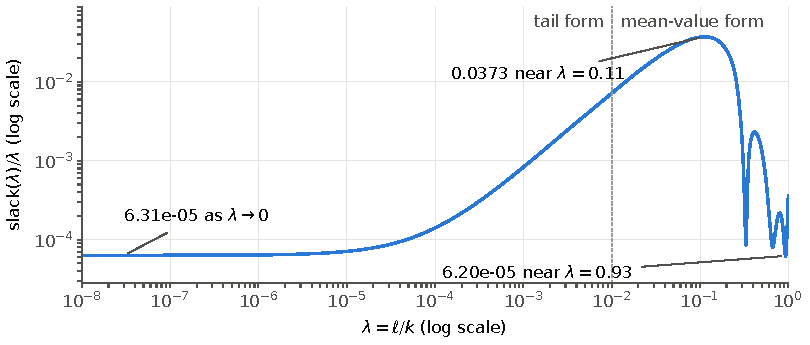
\includegraphics[width=\linewidth]{fig/ramsey-chain-slack.pdf}
\caption{Round~1: the slack of Theorem~\ref{thm:14}'s inequality divided by $\lambda$, as the lower end of an interval enclosure at each of \CurveN{} points (the decision is the cover of Table~\ref{tab:intervals}, not these points). It is flat near \SlackLim{} for small $\lambda$, rises to \SlackMax{} near $\lambda=\SlackMaxAt$, falls to \SlackMin{} near $\lambda=\SlackMinAt$, and ends at \SlackAtOne{} at $\lambda=1$. The flat left end and the three dips between $0.6$ and $0.95$ are where a coarser witness, or a slightly more ambitious $q$, is refused; the control that moves the linear coefficient to $-0.3870$ fails at the left end.}\label{fig:slack}
\end{figure}

The margins are thin and that is the content of the result. In round~1 the slack is about $\SlackLimM\,\lambda$ as $\lambda\to0$ and $\SlackMinM\,\lambda$ near $\lambda=\SlackMinAt$ (Figure~\ref{fig:slack}); the worst main interval of program 1 is $[\WorstLo,\WorstHi]$ with certified lower bound \MinMainLowerOne. The later rounds are proposed at margin $\delta\lambda$ with $\delta=\DeltaMarginM$ and decided at the certified lower bounds of Table~\ref{tab:intervals}.

\subsection{The float sequences, and where the iteration goes}\label{sec:float}

The proposer, run on its own and never decided, iterates past the certified rounds. Table~\ref{tab:float} and Figure~\ref{fig:rounds} record its sequences at degree six (\FloatSixIters{} iterations) and degree nine (\FloatNineIters{} iterations), each round in the float region of the round before, with the same margin $\delta$. Degree six settles near $\FloatSixSettle$ (last step \FloatSixDrop); degree nine near $\FloatNineSettle$ (last step \FloatNineDrop), and the certified round~\NRounds{} lies \FloatNineBeyond{} above the last float iterate. These are observations in floating point about the shape of the iteration, not bounds: they say that further rounds of this kind, in this parametrisation of $F$, would move the base by less than $10^{-5}$. The authors of \cite{GNNW} expect that going below $3.75$ needs new ideas; nothing here disagrees.

\begin{table}[h]\centering\small
\begin{tabular}{rll}\toprule
iteration & degree 6 (float, not decided) & degree 9 (float, not decided)\\\midrule
\FloatRows
\bottomrule\end{tabular}
\caption{The float proposer's bases, iteration $0$ being $\GAI$. Rounds $2$--$\NRounds$ of Theorem~\ref{thm:chain} are iterations $1$--$\NNew$ of the degree-9 column, rounded to six decimals and decided.}\label{tab:float}
\end{table}

\begin{figure}[h]\centering
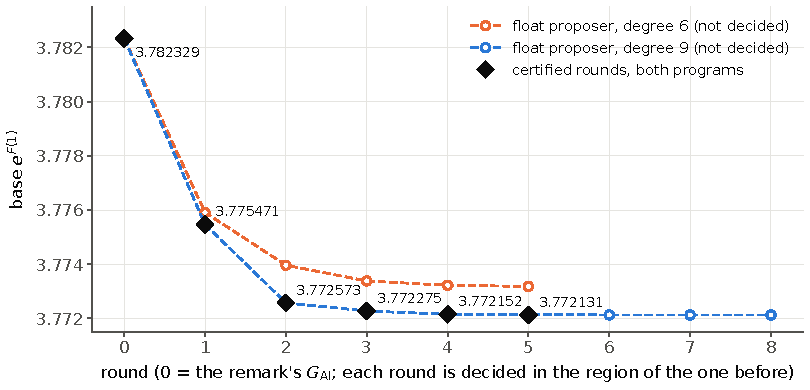
\includegraphics[width=\linewidth]{fig/ramsey-chain-rounds.pdf}
\caption{The certified bases of the \NRounds{} rounds (filled diamonds, both programs) beside the float proposer's sequences (hollow markers on dashed lines, never decided). Decided and proposed values share neither colour nor mark.}\label{fig:rounds}
\end{figure}

\section{The HorizonMath certificate}\label{sec:hm}

\subsection{The problem and the certificate}

HorizonMath \cite{HM} (version \HmArxiv, pinned by sha256 \HmSha\ldots; its code at commit \HmCommit{} of \texttt{github.com/\allowbreak ewang26/\allowbreak HorizonMath}) states the problem in the framework of Theorem~\ref{thm:14}, with $F(\lambda)=h(\lambda)+p(\lambda)e^{-\lambda}$ for a polynomial $p$ without constant term and $c=e^{F(1)}$, and verifies the condition $(X,Y)\in R$ through an inner approximation: a rate function
\[
U(\mu)=h(\mu)+\bigl(\HmUcubic\bigr)e^{-\mu},
\]
a set of pairs with $-\log x-\mu\log y\ge U(\mu)$ for all $\mu\in(0,1]$ --- the problem calls it $R_0$; we write $\Rz'$ to keep it apart from the $\Rz$ of \eqref{eq:R0} --- and the rule, in the problem's words, ``Since $R(k,\ell)=R(\ell,k)$, the pair $(x,y)$ is accepted if either $(x,y)\in R_0$ or $(y,x)\in R_0$.'' The function $U$ is $F_{0.033}$, the third stage of the iteration in the first version of \cite{GNNW}; it is a weaker bound than Theorem~1's $F_{0.03}$ and is implied by it, so the problem's inner approximation rests on a proved bound.

The certificate credited to \HmClaimant{} is printed as code (Appendix~A.3 of \cite{HM}) and was rebuilt here from that recipe. Its polynomial is
\[
p(\lambda)=\sum_{j=1}^{5}c_j\lambda^j,\qquad (c_1,\dots,c_5)=\HmCoeffs,
\]
the cubic of $U$ plus $\HmQuintic\,\lambda^5$; $M$ and $Y$ are constant on \HmIntervals{} intervals of $(\HmLambdaZero,1]$, with $Y$ set on each interval to $(1-\HmShrink)\min\{1,\,e^{-U(1)}/X\}$ at the interval's left end, in the certificate's own words ``\HmShrinkPct{} below the active $xy=e^{-U(1)}$ branch''. The benchmark's checker accepts it and reports $c=e^{F(1)}=\HmCPrinted$ (its whole output: ``\HmCheckerOutput''); the paper prints $c=\HmC\ldots$; our enclosure of $e^{F(1)}$ reproduces the digits, $[\HmCEncLo\ldots]$.

\subsection{Two inequalities, and a rule that asks for one}

A bound $R(k,\ell)\le e^{U(\ell/k)k+o(k)}$ is known for $\ell\le k$. By Observation~10(4) of \cite{GNNW} it places $(x,y)$ in $R$ when $R(k,\ell)\le x^{-k-o(k)}y^{-\ell-o(\ell)}$ for \emph{all} $k,\ell$, that is when, for every $s\in(0,1]$,
\begin{align}
-\log x-s\log y&\ \ge\ U(s)\qquad\text{(the pairs with $\ell\le k$),}\label{eq:line1}\\
-\log y-s\log x&\ \ge\ U(s)\qquad\text{(the pairs with $\ell>k$, read through $R(k,\ell)=R(\ell,k)$).}\label{eq:line2}
\end{align}
Lemma~\ref{lem:15} proves both before it places a point. The problem's $\Rz'$ is \eqref{eq:line1} alone, and its rule accepts $(x,y)$ when \eqref{eq:line1} holds \emph{or} \eqref{eq:line2} holds. Symmetry of $R(k,\ell)$ makes $R$ symmetric; it does not make a one-sided test two-sided. The consequence is concrete. $U$ increases on $(0,1]$ (as in (35) of \cite{GNNW}, $U'\ge\log2-\tfrac14$), so \eqref{eq:line1} holds for every $y$ as soon as $-\log x\ge U(1)$, i.e.\ $x\le e^{-U(1)}=\HmEUlong\ldots$ --- the certificate's own constant $c_{\mathrm{hyp}}=\HmChyp$. The rule therefore accepts the whole strip $\{x\le\HmEU\}\times(0,1)$, for instance $(0.26,0.9999)$, which $R$ cannot contain (Lemma~\ref{lem:erdos} below). The certificate places its pairs on that strip wherever $X$ is small, and $X(1)=\HmLastX$ is.

\subsection{The exclusion}

\begin{lemma}[Erd\H{o}s \cite{Erd47}, first moment]\label{lem:erdos}
For $k,m\ge3$ and $0<p<1$ let $N=\lfloor\min(p^{-(k-1)/2},(1-p)^{-(m-1)/2})\rfloor$. Then $R(k,m)>N$. Consequently, if $(x,y)\in R$, then for every $e>0$ and $0<p<1$,
\[
e\,(-\log x)+(-\log y)\ \ge\ \min\bigl(\tfrac e2(-\log p),\ \tfrac12(-\log(1-p))\bigr),
\]
and the same with $x$ and $y$ exchanged.
\end{lemma}
\begin{proof}
Colour $K_N$ red with probability $p$ independently. The expected number of red $K_k$ is at most $N^kp^{\binom k2}/k!\le1/6$ and of blue $K_m$ at most $1/6$, so some colouring has neither. For the consequence, let $(x,y)\in R$ and $d>0$; since $R$ is the closure of $\Rz$ and $\Rz$ is closed downward, $(x-d,y-d)\in\Rz$, so $N<R(k,m)\le(x-d)^{-k}(y-d)^{-m}$ for all large $k+m$. Take $k=\lceil em\rceil$, divide the logarithms by $m$, let $m\to\infty$ and then $d\to0$. The exchanged form is the regime $m=\lceil ek\rceil$.
\end{proof}

The decision is one rational pair $(e,p)$ per point: the lower end of an enclosure of the right side exceeds the upper end of an enclosure of the left side, in decimal intervals of 60 digits with every rounding outward (\texttt{instruments/\allowbreak horizonmath/\allowbreak ramsey\_region.py}, written from the two papers and sharing no code with the benchmark's validator). A float search proposes $(e,p)$; the interval comparison is the authority. At $\lambda=1$, with $e=\HmE$ and $p=\HmP$ in the regime $k=\lceil em\rceil$, Erd\H{o}s's rate is at least $\HmErdosLo$ per $m$ while the pair allows at most $\HmPairHi$: a gap of $\HmGap$. The pair is not in $R$; the second hypothesis of Theorem~\ref{thm:14} fails at the point where $c=e^{F(1)}$ is read; Proposition~\ref{prop:hm} follows.

Across the certificate (Figure~\ref{fig:region}, Table~\ref{tab:hm}): \HmOutside{} of \HmPoints{} points are outside $R$, each with its own $(e,p)$ --- among them the first interval, at $\lambda=\HmFirstLambda$, where $(X,Y)=(\HmFirstX,\HmFirstY)$ is excluded with $e=\HmFirstE$, $p=\HmFirstP$; \HmNotPlaced{} more are shown by one rational $s$ at which $U(s)$ exceeds the line \eqref{eq:line1} or \eqref{eq:line2} not to be placed in $R$ by the problem's own $U$ (they may or may not lie in $R$ by some other bound); and \HmNotRefuted{} are not refuted here, the points with $\lambda\in[\HmNrLamLo,\HmNrLamHi]$ and $X\in[\HmNrXLo,\HmNrXHi]$, near the window $[\HmAone,\HmBone]$ where the hyperbola branch of Lemma~\ref{lem:15} is legitimate for $f=U$ (that window is computed in floating point for the figure and is not part of any verdict).

\begin{figure}[h]\centering
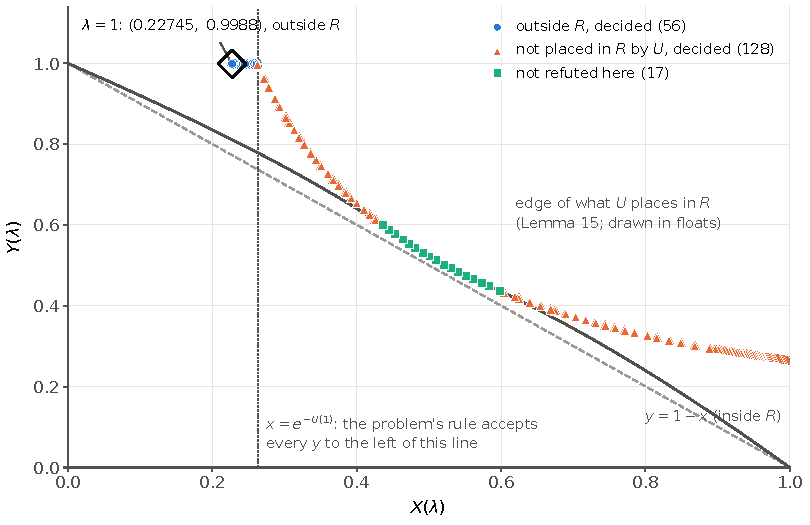
\includegraphics[width=\linewidth]{fig/ramsey-chain-region.pdf}
\caption{The certificate's \HmPoints{} pairs $(X(\lambda),Y(\lambda))$, each at the midpoint of an interval on which $M$ and $Y$ are constant, and $\lambda=1$ itself (the diamond). Marks and colours repeat the three verdicts, which are decided; the solid curve is the edge of what $U$ places in $R$ by Lemma~\ref{lem:15}, drawn in floats and not decided; the dashed diagonal $y=1-x$ is inside $R$ by the Erd\H{o}s--Szekeres bound. Left of the dotted line $x=e^{-U(1)}$ the problem's rule accepts every $y$.}\label{fig:region}
\end{figure}

\begin{table}[h]\centering\small
\resizebox{\linewidth}{!}{%
\begin{tabular}{rrrll}\toprule
$\lambda$ & $X(\lambda)$ & $Y(\lambda)$ & decided & witness\\\midrule
\HmSampleRows
\bottomrule\end{tabular}}
\caption{Eight of the \HmPoints{} decided points, $X$ as the lower end of its enclosure. A witness $(e,p)$ excludes the pair from $R$ by Lemma~\ref{lem:erdos}; a witness $s$ shows the problem's $U$ does not place it.}\label{tab:hm}
\end{table}

\subsection{The checker, as published and with one token changed}

As an observation, recorded in the corpus and not part of any verdict: the benchmark's validator (\texttt{validators/\allowbreak ramsey\_asymptotic.py} at the pinned commit), run as published on \HmObservedOn, accepts the rebuilt certificate in \HmCheckerSeconds{} s. Its line \HmCheckerLine{} reads \texttt{\HmCheckerMin}, the better of the two orientations' margins; with \texttt{\HmCheckerMax} in its place, so that both orientations must clear their thresholds as membership in $R$ requires, it refuses the certificate in \HmWithAndSeconds{} s, on its first interval $[\HmFirstIntervalLo,\HmFirstIntervalHi]$. The defect is in the problem statement, which gives the either-orientation rule in words, and in its checker; the model optimised against the problem as stated, and the certificate reads as a faithful solution of that problem. The verification that relied on the checker is what the record contradicts.

\paragraph{Controls.} The battery for this ledger (\HmBattery{} checks, \HmRed{} red controls, four of them on this row) requires that the 99 Erd\H{o}s--Szekeres pairs $(j/100,1-j/100)$ and the forty points $(X_0,1-X_0)$ of Lemma~16(1) of \cite{GNNW} are never excluded from $R$ nor left unplaced by $U$; that $(e^{-U(1)}-10^{-6},0.9999)$, which the rule accepts, is excluded; that the certificate's pair at $\lambda=1$ is excluded; and that a float proposer claiming $(\tfrac12,\tfrac12)$ outside $R$, or unplaced by $U$, is overruled by the interval check. The same ledger decides the benchmark's other printed construction, a 128-triangle Kakeya set, whose union area is exactly $\KakeyaNum/\KakeyaDen=\KakeyaDec\ldots$ (CERTIFIED), and records the three closed forms it credits to a second model as NEEDS DATA because they are not printed; neither is in this paper's scope.

\section{What is not claimed}

\begin{itemize}
\item Theorem~14, Lemma~15 and Theorem~1 of \cite{GNNW} are used, not re-proved, and the $o(k)$ in Theorem~\ref{thm:chain} is theirs, including its uniformity in $\ell\le k$ on which the induction through Lemma~15 depends. Round $i$ rests on the bound round $i-1$ establishes; the chain is as strong as its first link, which is the paper's Theorem~1.
\item Nothing here is the best known bound on $R(k,k)$. Theorem~\ref{thm:chain} continues the iteration of \cite{GNNW}; $R(k,k)\le3.769^{\,k+o(k)}$ \cite{NSS26} and $R(k,k)\le3.69507^{\,k}$ \cite{LW26} are lower, and neither is checked here.
\item No inequality about Ramsey numbers is refuted. Proposition~\ref{prop:hm} refutes a certificate: whether $R(k,k)\le(\HmCFour\ldots)^{k+o(k)}$, or any base below $3.7992$, holds is untouched by it (the bound of \cite{LW26}, not checked here, would imply the former). Whether some certificate of the benchmark's quintic form, with pairs inside $R$, beats $3.7992$ is open; the Erd\H{o}s bound alone does not exclude the quintic $F$ of Section~\ref{sec:hm} for every $M$.
\item Nothing is claimed about optimality. The float observation of Section~\ref{sec:float} concerns this parametrisation of $F$ and this proposer; a different family of $F$, or a different $M$, is not excluded by it.
\item The two programs are independent in language, arithmetic and bounding method, but share an author and a reading of the paper. A check by the authors of \cite{GNNW}, or by anyone running the one-file verifier, is the next step; nothing has been sent to the authors of either paper.
\item This document is machine-derived and not peer-reviewed. Every number in it is interpolated from the records named below; the author asserts nothing numerical beyond what they hold.
\end{itemize}

\paragraph{Points for review.} (i) The reading of Theorem~14's hypothesis ``$F:(0,1]\to\mathbb R_+$ smooth'' as satisfied by $h+qe^{-\lambda}$ with positivity implied by the strict inequality. (ii) Whether the hypotheses of Lemma~15 decided for each $F_{i-1}$ (Section~\ref{sec:framework}) are all of them, and whether applying the lemma to a bound obtained from Theorem~14 (uniform $o(k)$) is exactly its hypothesis (29). (iii) The reading of the remark as the statement that Theorem~14's hypotheses can be met for $F=h+\GAI$ with $Y$ from Remark~17 --- the remark names no $M$ or $Y$, so a different reading would decide a different claim. (iv) The reading of $R$ as two-sided, on which Proposition~\ref{prop:hm} turns; it is the definition (12) of \cite{GNNW} and the practice of its Lemma~15. (v) The record's reproduction line names the verifier as \texttt{verify/verify\_gnnw\_gai.py}; the file is at \texttt{tools/verify\_gnnw\_gai.py}, and the sha256 above is of that file.

\cmrepro{The records:
\begin{itemize}\setlength{\itemsep}{0pt}
\item \texttt{certs/gnnw-certificate.json} --- round~1, generated \ZGenerated;
\item \texttt{certs/gnnw-chain-certificate.json} --- the \NRounds{} rounds, both programs, generated \KGenerated{} (the second program's run of \SecondRan{} is \texttt{corpus/gnnw/second-run.json}, pinned by the sha256 of its code and of the chain);
\item \texttt{certs/horizonmath-ledger.json} --- the benchmark's certificate, generated \LGenerated.
\end{itemize}
The corpus is \texttt{corpus/gnnw} --- the paper arXiv \GnnwArxiv{} pinned by sha256 \GnnwSha\ldots{} and its version 1 by \GnnwVoneSha\ldots, neither stored; the remark transcribed; the witness nodes; the chain, sha256 \ChainSha\ldots{} --- and \texttt{corpus/horizonmath} --- the paper and the benchmark's code pinned, not stored; the printed recipe transcribed and the certificate rebuilt from it by \texttt{rebuild\_ramsey\_a3.py}. From the repository root (commit \RepoCommit):
\begin{itemize}\setlength{\itemsep}{0pt}
\item round~1 with the standard library alone, about \SecondsOne{} s:\\ {\small\texttt{python3 tools/verify\_gnnw\_gai.py certs/gnnw-certificate.json}}
\item the chain, about \SecondsChainPy{} s:\\ {\small\texttt{python3 tools/verify\_gnnw\_gai.py certs/gnnw-chain-certificate.json}}
\item the second program, about \MinutesChainJs{} minutes:\\ {\small\texttt{node instruments/gnnw/second.js corpus/gnnw/chain.json}}
\item re-derive both records: {\small\texttt{python3 tools/run-gnnw-ledger.py --check}}
\item the \GnnwBattery{} checks and \GnnwRed{} refused forgeries: {\small\texttt{python3 instruments/gnnw/battery.py}}
\item the benchmark's ledger re-derived: {\small\texttt{python3 tools/run-horizonmath-ledger.py --check}}
\item its \HmBattery{} checks: {\small\texttt{python3 instruments/horizonmath/battery.py}}
\item the proposer (numpy and scipy); its second file reproduces the chain byte for byte:\\ {\small\texttt{instruments/gnnw/propose/iterate2.py}}, {\small\texttt{instruments/gnnw/propose/buildchain.py}}
\item the macros and the figures of this document, from the records, and the document itself:\\ {\small\texttt{node tools/paper-numbers/ramsey-chain.js}}\\ {\small\texttt{instruments/hseva/.venv/bin/python tools/paper-numbers/ramsey-chain-figs.py}}\\ {\small\texttt{node tools/build-paper-tex.js ramsey-chain}}
\end{itemize}
Pages built from the same records: {\small\url{https://carlostoledo.co/reports/diagonal-ramsey.html}} and {\small\url{https://carlostoledo.co/reports/horizonmath.html}}.}

\begin{thebibliography}{99}\small
\bibitem{Ram30} F.~P. Ramsey, On a problem of formal logic, Proc.\ London Math.\ Soc.\ (2) 30 (1930), 264--286.
\bibitem{ES35} P.~Erd\H{o}s, G.~Szekeres, A combinatorial problem in geometry, Compositio Math.\ 2 (1935), 463--470.
\bibitem{Erd47} P.~Erd\H{o}s, Some remarks on the theory of graphs, Bull.\ Amer.\ Math.\ Soc.\ 53 (1947), 292--294.
\bibitem{Tho88} A.~Thomason, An upper bound for some Ramsey numbers, J.\ Graph Theory 12 (1988), 509--517.
\bibitem{Con09} D.~Conlon, A new upper bound for diagonal Ramsey numbers, Ann.\ of Math.\ (2) 170 (2009), 941--960.
\bibitem{Sah23} A.~Sah, Diagonal Ramsey via effective quasirandomness, Duke Math.\ J.\ 172 (2023).
\bibitem{CGMS} M.~Campos, S.~Griffiths, R.~Morris, J.~Sahasrabudhe, An exponential improvement for diagonal Ramsey, arXiv:2303.09521 (2023).
\bibitem{GNNW} P.~Gupta, N.~Ndiaye, S.~Norin, L.~Wei, Optimizing the CGMS upper bound on Ramsey numbers, arXiv:2407.19026; version 2 of 29 August 2026, pinned by sha256 \GnnwSha\ldots{} (\texttt{corpus/gnnw/meta.json}); its main results are stated to be formalised in Lean~4 at \url{https://github.com/snorin239/RamseyLean}.
\bibitem{HM} E.~Y. Wang, S.~R. Motwani, J.~V. Roggeveen, E.~Hodges, D.~Jayalath, C.~London, K.~Ramakrishnan, J.~Foerster, C.~Zhang, F.~Cipcigan, P.~Torr, A.~Abate, Measuring AI progress toward mathematical discovery with automatic verification (HorizonMath), arXiv:2603.15617; version 2 of 10 September 2026, pinned by sha256 \HmSha\ldots; code at \url{https://github.com/ewang26/HorizonMath}, commit \HmCommit{} (\texttt{corpus/horizonmath/meta.json}).
\bibitem{NSS26} C.~Neisler, R.~M.~J. Shin, S.~Sukhatankar, A self-consistent bootstrap for the book algorithm and the bound $R(k,k)\le3.769^{k+o(k)}$, revision v3, 2 September 2026, with a Lean~4 formalization at \url{https://github.com/wamlat/RamseyLean-bootstrap}, archived at doi:10.5281/zenodo.22263823 (3 September 2026); README, Zenodo record and the paper source's sha256 pinned in \texttt{corpus/sources/ramsey}.
\bibitem{LW26} Z.~Lu, S.~Wang, Retained-Set Descent for Diagonal Ramsey Numbers, arXiv:2609.14525 (13 September 2026); the abstract page pinned in \texttt{corpus/sources/ramsey}.
\bibitem{Moore} R.~E. Moore, Interval Analysis, Prentice-Hall, 1966.
\bibitem{Tucker} W.~Tucker, Validated Numerics: A Short Introduction to Rigorous Computations, Princeton University Press, 2011.
\end{thebibliography}

\end{document}
